\section{Optimering}
For at optimere filteret anvendes et andet vindue. Ved at eksperimentere med de forskellige vinduer ses det, at der også opstår ripples ved Blackman-vinduet, hvorimod anvendelser af Hann- og Hamming-vinduet giver ingen eller meget små ripples. Eksempler på dette er vist i figur \ref{fig:filter_Hann_Hamming}.
\begin{figure}[H]
\begin{minipage}{0.49\textwidth}
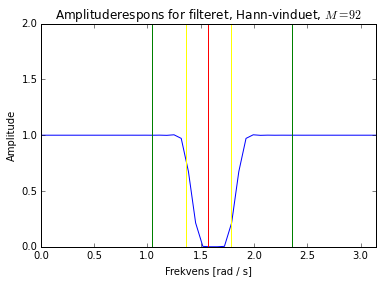
\includegraphics[width=0.9\textwidth]{figures/Filter_Hann_92.PNG}
\end{minipage}
\begin{minipage}{0.49\textwidth}
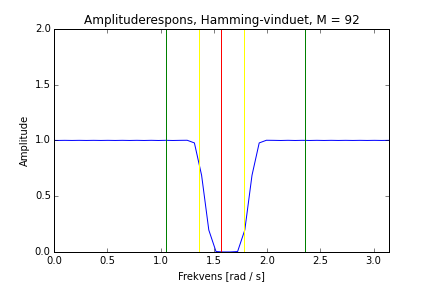
\includegraphics[width=0.9\textwidth]{figures/Filter_Hamming_92.PNG}
\end{minipage}
\caption{Eksempler på båndstopfilteret ved hjælp af det rektangulære vindue og med forskellige filterordener $M$. De to grønne streger markerer $\omega_1$ og $\omega_3$, som skal beholdes, og de to gule streger markerer $\omega_{c_1}$ og $\omega_{c_2}$, som ligger symmetrisk omkring den røde streg, der markerer $\omega_2$, som skal elimineres.}
\label{fig:filter_rekt}
\end{figure}